\begin{theorem}[The First Isomorphism Theorem] \leavevmode \\
    \label{thm16}
    If $\phi: G \to H$ is a group homomorphism, then $\ker\phi \nsubgroup G$ and 
    $$G/ker\phi \cong \phi(G) \leq H$$
\end{theorem}

\begin{corollary}
    Let $\phi: G \to H$ be a group homomorphism.
    \begin{enumerate}
        \item $\phi$ is injective if and only if $\ker\phi = \set{1}$
        \item $|G:\ker\phi| = |\phi(G)|$
    \end{enumerate}
\end{corollary}

\begin{theorem}[The Second Isomorphism Theorem; The Diamond Theorem] \leavevmode \\
    \label{thm18}
    Let $G$ be a group and let $A, B \leq G$. Assume $A \leq N_G(B)$. Then 
    \begin{align*}
        AB &\leq G \\
        B &\nsubgroup AB \\
        A\cap B &\nsubgroup A \\
        AB/B &\cong A/A\cap B
    \end{align*}
    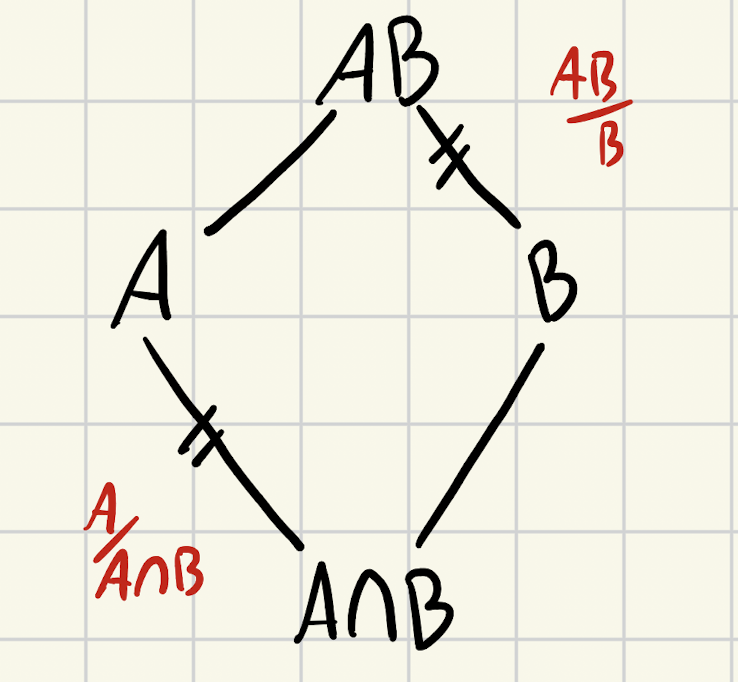
\includegraphics[width= 100pt, center]{/Users/josiahvillarante/GradSchool/Grad-School-Notes/Math210A/CH3/images/Diamond Thm.png}
\end{theorem}

\begin{proof}
    Since $A \leq N_G(B), B \leq N_G(B),$ it follows that 
    $$AB \leq N_G(B)$$
    and since $B \leq AB$, we have $B \nsubgroup AB.$

    Since $B \nsubgroup AB,$ then $AB/B$ is a group. Define 
    \begin{align*}
        \phi: A &\to AB/B \\
        \phi(a) &= aB ~~\forall a \in A
    \end{align*}
    By the First Isomorphism Theorem, if $\phi$ is a homomorphism then 
    $$A/\ker\phi \cong \phi(A)$$

    We need to show 
    \begin{enumerate}
        \item $\phi$ is a homomorphism
        \item $\phi(A) = AB/B$
        \item $\ker\phi = A\cap B$
    \end{enumerate}

    1. Let $a_1, a_2 \in A$. Then 
    \begin{align*}
        \phi(a_1a_2) &= a_1a_2B \\
        &=(a_1B)(a_2)B \\
        &=\phi(a_1)\phi(a_2)
    \end{align*}

    2. Notice that $abB = aB$ since $b\in B$. That is, $\forall abB \in AB/B ~~abB = aB.$ Thus our mapping is surjective. Hence $\phi(A) = AB/B.$
    \\ \\
    3. Notice 
    \begin{align*}
        \ker\phi &= \set{a \in A : \phi(a) = 1B} \\
        &= \set{a \in A : aB = 1B} \\
        &= \set{a \in A : a \in B} \\
        &= A \cap B
    \end{align*}

    By the First Isomorphism Theorem on 1, 2, and 3, we have $A/\ker\phi \cong \phi(A)$. That is,
    $$A/A\cap B \cong AB/B$$
    where $A\cap B \nsubgroup A.$
    \qed
\end{proof}

\begin{theorem}[The Third Isomorphism Theorem] \leavevmode \\
    \label{thm19}
    Let $G$ be a group and let $H$ and $K$ be normal subgroups of $G$ with $H \leq K.$ Then 
    $$\frac{G/H}{K/H} \cong G/K$$
\end{theorem}

\begin{proof}
    We proceed to define a homomorphism from $G/H \to G/K$ that is surjective such that $\ker\phi = K/H$. Then the claim follows fro the First Isomorphism Theorem. \\

    Since $K\nsubgroup G, \pi_H(G) = \set{kH : k \in K}.$ We know that the 
    $$\pi_H(K) \nsubgroup \pi_H(G) = G/H$$
    Notice $\set{kH : k \in K} = K/H.$ Define 
    \begin{align*}
        \phi: G/H &\to G/K \\
        gH &\mapsto gK ~~\forall g \in G
    \end{align*}

    We proceed to show $\phi$ is a well-defined, epimorphism (surjective homomorphism).

    \begin{description}
        \item[$\phi$ is well-defined: ] Suppose $g_1H = g_2H$. Then $g_1 = g_2 h$ for some $h \in H.$ Since $H \leq K$, $h \in K.$ That is 
        \begin{align*}
            &g_1 = g_2h \text{ where } h \in K \\
            \implies &g_1K = g_2K
        \end{align*}
        Hence $\phi(g_1H) = \phi(g_2H)$ and our function is well-defined.

        \item[$\phi$ is a homomorphism: ] Let $g_1H, g_2H \in G/H$. Then 
        \begin{align*}
            \phi(g_1Hg_1H) &= \phi(g_1g_2H) \\
            &= g_1g_2K \\
            &= (g_1K)(g_2K) \\
            &= \phi(g_1H)\phi(g_2H)
        \end{align*}
        Hence, $\phi$ is a homomorphism.

        \item[$\phi$ is surjective: ] $\phi$ is clearly surjective by construction. 

        \item[$\ker\phi = K/H$: ]
        \begin{align*}
            \ker\phi &= \set{gH \in G/H : \phi(gH) = 1K} \\
            &= \set{gH \in G/H : gK = 1K} \\ 
            &= \set{gH \in G/H : g \in K} \\
            &= K/H
        \end{align*} 
    \end{description}
    By the First Isomorphism Theorem, 
    $$\frac{G/H}{K/H} \cong G/K$$
    \qed
\end{proof}

\begin{theorem}[The Fourth Isomorphism Theorem; The Lattice Isomorphism Theorem] \leavevmode \\
    \label{thm20}
    Let $G$ be a group with $N \nsubgroup G$. Then there is a bijection from $\set{A \leq G : N \leq A}$ to the set of subgroups of $G/N$. In particular, every subgroup of $\overline{G} = G/N$ is of the form $\overline{A} = A/N$ for some subgroup $A$ of $G$, containing $N$ (Namely, the complete preimage of the subgroup of $G/N$, under the natural projection from $G$ to $G/N$). \\

    This bijection has the following properties:
    \begin{enumerate}
        \item $A\leq B \iff \overline{A} \leq \overline{B}$ ($A/N \leq B/N$)
        \item If $A \leq B$ then $|A:B| = |B/N : A/N| = |\overline{B} : \overline{A}|$
        \item $\overline{<A,B>} = <\overline{A}, \overline{B}>$
        \item $\overline{A\cap B} = \overline{A} \cap \overline{B}$
        \item $A \nsubgroup G \iff \overline{A} \nsubgroup \overline{G}$
    \end{enumerate}
\end{theorem}

\begin{example}
    The group $Q_8:$

    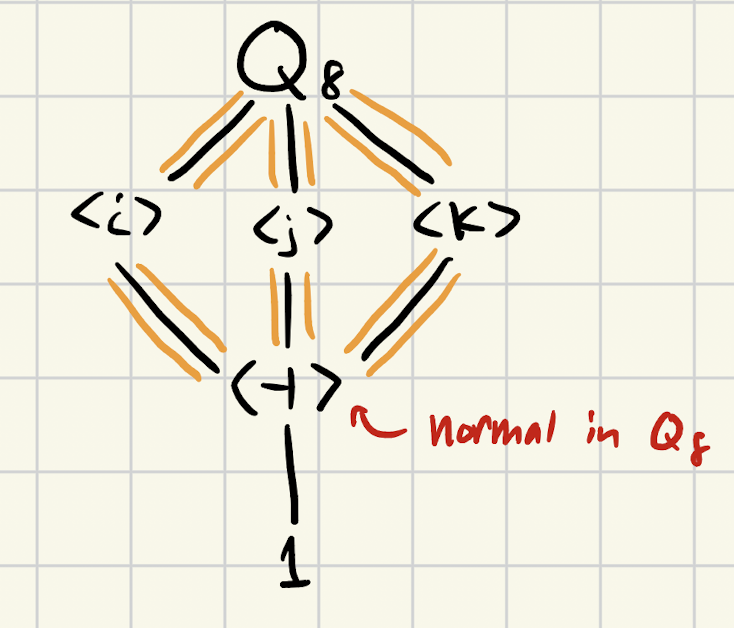
\includegraphics[width= 100pt, center]{/Users/josiahvillarante/GradSchool/Grad-School-Notes/Math210A/CH3/images/Q8 Lattice.png}

    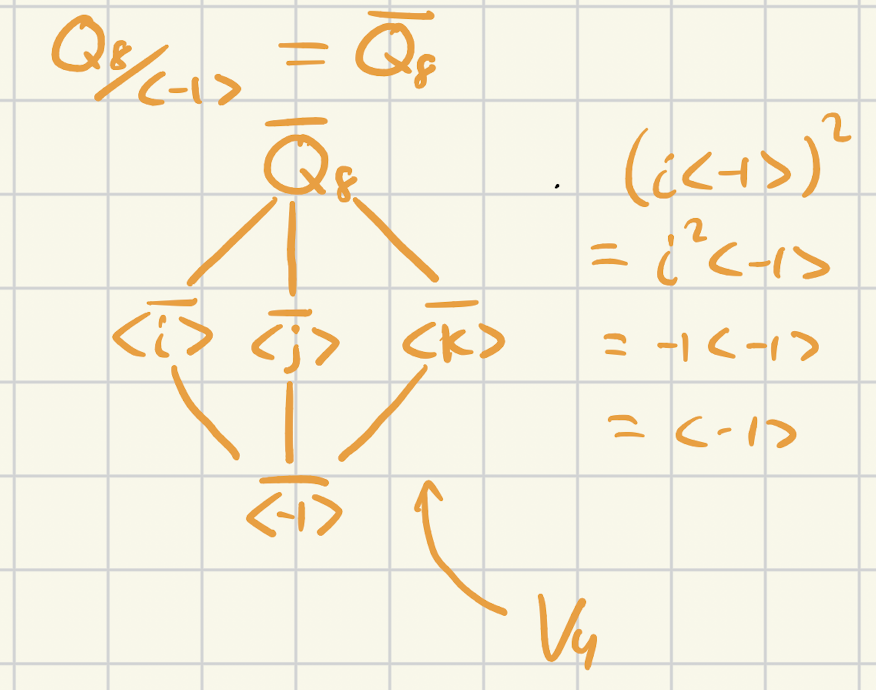
\includegraphics[width= 100pt, center]{/Users/josiahvillarante/GradSchool/Grad-School-Notes/Math210A/CH3/images/Q8 Lattice 2.png}
\end{example}